\documentclass[aspectratio=169,12pt,xcolor={table},compress]{beamer}
\usepackage{verbatim}
\usepackage{graphicx}
\usepackage{hyperref}
\usepackage{hulipsum}
\usepackage{enumerate}
\usepackage{tikz}
\usepackage{movie15}
\usepackage{animate}
\usepackage{listings}
\usepackage{xcolor}

\newtheorem{tet}{Naprendszerünk központja}
\newtheorem{tet1}{Tétel}
\newcommand{\no}[1]{\mathbf{n}_{#1}}
\newcommand{\n}{\mathbf{n}}
\newcommand{\co}{\mathbf{c}}

\author{Sindely Richárd}
\title{A Naprendszer}
\date{2023}

\useinnertheme[shadow=true]{rounded}
\useoutertheme{miniframes}
\usefonttheme{serif}
\usecolortheme{albatross}

\begin{document}
\frame{\titlepage}
\section{Kezdetek}
\subsection{Fiatal naprendszer}
\frame{\tableofcontents[currentsection]}
\begin{frame}{A naprendszer keletkezése}
\begin{columns}[c]
\begin{column}{.5\linewidth}
A Naprendszer 4,6 milliárd évvel ezelőtt egy csillagközi gáz- és porfelhőből alakult ki. A felhő sűrűsödésnek indult, egyre több anyag gyűlt össze a középpontjában, amely egyre forróbb lett, majd kialakult az ősi Nap. A megmaradt anyag korong alakba csoportosult. A korongban lévő anyagból keletkeztek az úgynevezett bolygócsírák\footnote{pl. kisbolygók, üstökösök}. Az ütközésük hatására jöttek létre bolygók és holdjai.
\end{column}
\begin{column}{.5\linewidth}
\begin{figure}
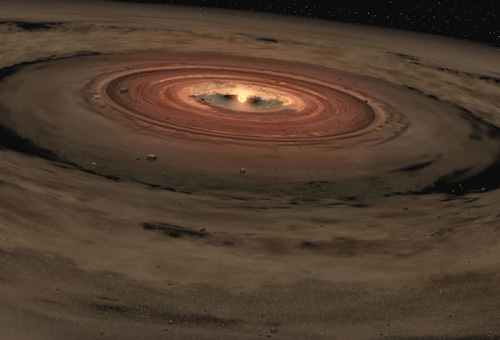
\includegraphics[height=5cm,width=7cm]{D:/Uni/Tex/Beadandó/fiatal_naprendszer.jpg}
\caption{Fiatal naprendszer}
\end{figure}
\end{column}
\end{columns}
\end{frame}
\subsection{Naprendszer napjainkban}
\begin{frame}{Naprendszer napjainkban}
\begin{columns}[c]
\begin{column}{.5\linewidth}
A naprendszer központja a nap és megtalálható benne 8 bolygó:
\begin{itemize}
\item<1> Merkúr
\item<2> Vénusz
\item<3> Föld
\item<4> Mars
\item<5> Jupiter
\item<6> Szaturnusz
\item<7> Uránusz
\item<8> Neptunusz
\transdissolve<1,2,3,4,5,6,7,8>
\end{itemize}
\end{column}
\begin{column}{.5\linewidth}
\begin{figure}
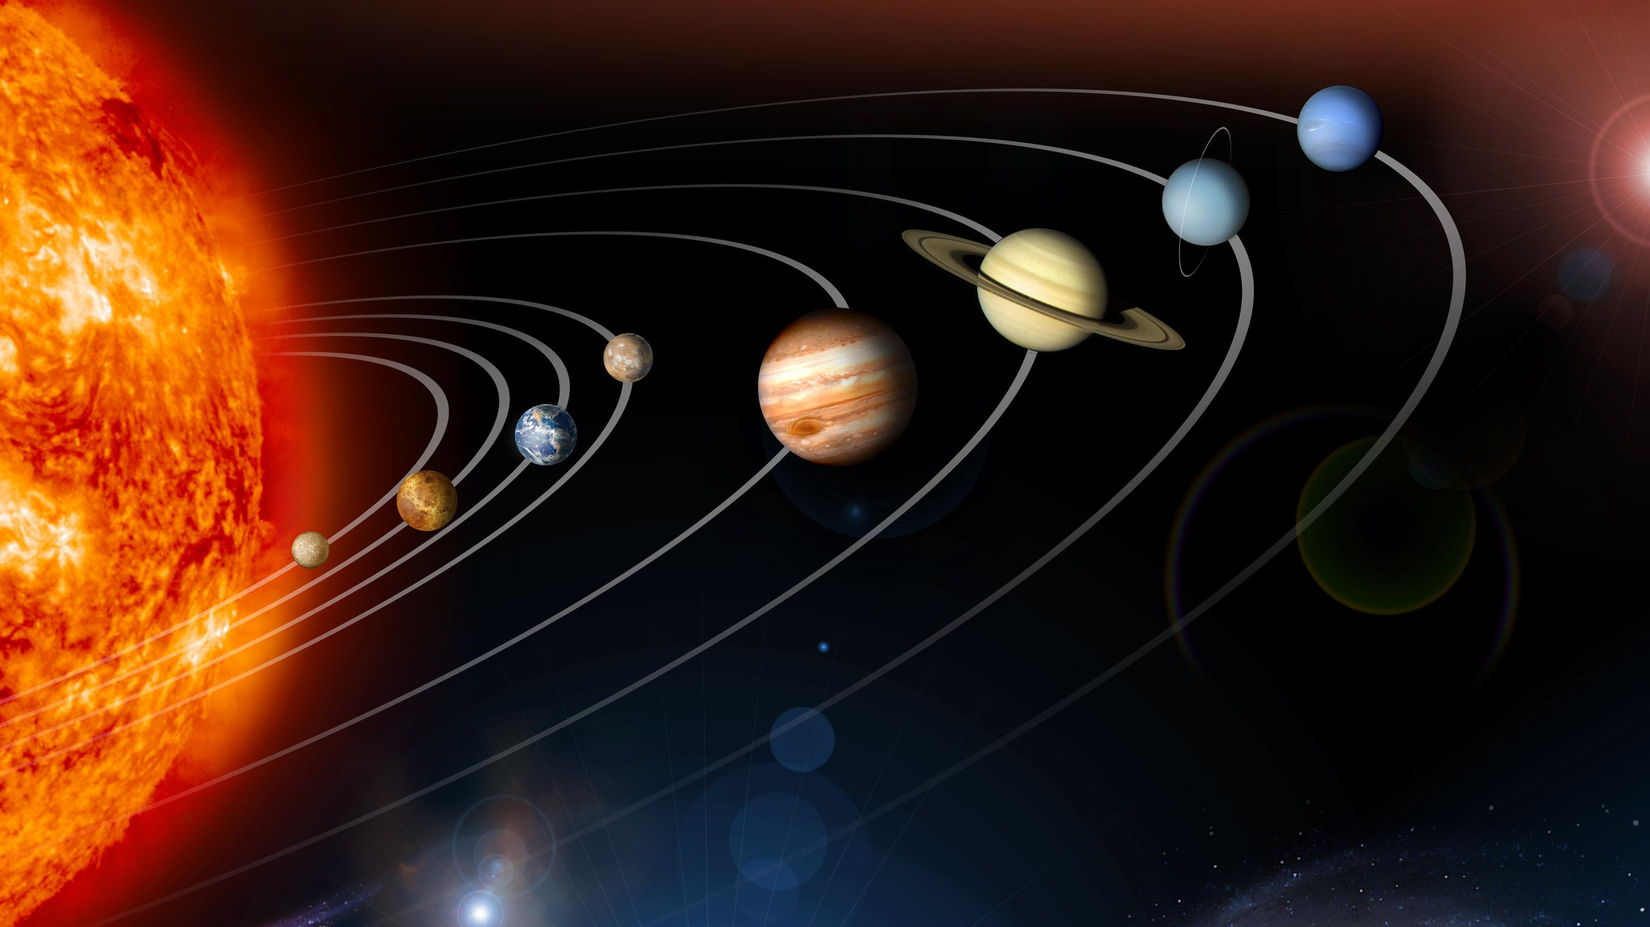
\includegraphics[height=5cm,width=7cm]{D:/Uni/Tex/Beadandó/naprendszer.jpg}
\caption{Naprendszer napjainkban}
\end{figure}
\end{column}
\end{columns}
\end{frame}
\begin{frame}{Bolygók legfőbb adatai}
\resizebox{14cm}{!}{
\begin{tabular}{|c|c|c|c|}
\hline
Bolygó neve & Legkisebb távolsága a Naptól & Legnagyobb távolsága a Naptól & Holdjainak darabszáma \\ \hline
Merkúr & 46 001 272 km & 69 817 079 km & nincs \\ \hline
Vénusz & 107 476 002 km & 108 941 849 km & nincs \\ \hline
Föld & 147 098 074 km & 152 097 701 km & 1 db \\ \hline
Mars & 206 644 545 km & 249 228 730 km & 2 db \\ \hline
Jupiter & 740 742 598 km & 816 081 455 km & 67 db \\ \hline
Szaturnusz & 1 349 467 375 km & 1 503 983 449 km & 62 db \\ \hline
Uránusz & 2 735 555 035 km & 3 006 389 405 km & 27 db \\ \hline
Neptunusz & 4 459 631 496 km & 4 536 874 325 km & 14 db \\ \hline
\end{tabular}
}
\end{frame}
\section{Naprendszer}
\frame{\tableofcontents[currentsection]}
\subsection{Nap}
\begin{frame}{Nap}
\begin{columns}[c]
\begin{column}{.5\linewidth}
\only<1-2>{
\begin{tet}
A Nap a naprendszer központi csillaga, körülötte keringenek az égitestek. 73.5\%-ban hidrogénből áll amely magfúzió során héliummá alakul. A folyamat során felszabaduló energia a fény. A Nap 4.57 milliárd éves. Ha fűtőanyaga elfogy, akkor a mérete az eredeti méretéhez képest százszorosára is megnőhet, vörös óriás lesz belőle elnyelve az összes bolygót ami az útjába kerül.
\end{tet}}
\only<3-4>{
Belső felépítése belülről kifelé haladva:
\begin{itemize}
\item Mag
\item Korona
\item Fotoszféra
\item Napkitörések
\end{itemize}
Napkitörések nap mint nap folynak a nap külső rétegén és egy-egy napkitőrés akár a föld méretétől nagyobb is lehet. Ha eltalál minket egy nagyobb napkitörés maximum csak áramkimaradást tud okozni.
}
\end{column}
\begin{column}{.5\linewidth}
\begin{figure}
\includegraphics<4>[height=5cm,width=7cm]{D:/Uni/Tex/Beadandó/napreteg.png}\transdissolve<4>
\includegraphics<2>[height=5cm,width=7cm]{D:/Uni/Tex/Beadandó/nap.jpg}\transdissolve<2>
\end{figure}
\only<1>{
\begin{center}
\begin{tikzpicture}[x=0.3cm,y=0.3cm]
\draw (5,0)
arc (0:360:5);
\foreach \angle in { 0,45,...,360 }{
\draw [rotate around={\angle:(0,0)}]
(5.5,0)    
-- +(0,-1.5)
-- +(3,0)
-- +(0,1.5)
-- cycle;
}
\end{tikzpicture}
\end{center}}
\end{column}
\end{columns}
\end{frame}
\subsection{Kőzetbolygók}
\subsubsection{Merkúr}
\frame{\tableofcontents[currentsection]}
\begin{frame}{Merkúr}
\begin{columns}[c]
\begin{column}{.5\linewidth}
Merkúr a legkisebb bolygó a naprendszerben és a naphoz legközelebbi bolygó. Földhöz hasonlóan \textbf{kőzetbolygó}. Felszíne a holdhoz hasonló, kráterekkel borított, illetve vulkanikus síkságok tagolják, de vannak a felszínén gyűrődések és völgyek is. A nap körüli keringési idő 87.97 nap.
\end{column}
\begin{column}{.5\linewidth}
\begin{figure}
\includegraphics<2>[height=4cm,width=7cm]{D:/Uni/Tex/Beadandó/merkur.jpg}\transdissolve<2>
\end{figure}
\end{column}
\end{columns}
\end{frame}
\subsubsection{Vénusz}
\begin{frame}{Vénusz}
\begin{columns}[c]
\begin{column}{.5\linewidth}
Legfényesebb égitestek közé tartozik. Második bolygó a naprendszerben amelyik a legközelebb kering a naphoz. \textbf{Közetbolygó}, méretében és tömegében is hasonlít a földhöz. Felszíne kietlen, sziklás. Bazaltvulkánok működnek a felszínén. Lemeztektonikai folyamatok nincsenek, kénsavcsepp-felhők rétegei takarják el a felszínt. A nap körüli keringési idő 224.7 nap. Holdjainak száma: 0, azaz nincsen holdja.
\end{column}
\begin{column}{.5\linewidth}
\begin{figure}
\includegraphics<2>[height=5cm,width=7cm]{D:/Uni/Tex/Beadandó/venusz.jpg}\transdissolve<2>
\end{figure}
\end{column}
\end{columns}
\end{frame}
\subsubsection{Föld}
\begin{frame}{Föld}
\begin{columns}[c]
\begin{column}{.5\linewidth}
Harmadik bolygó a naprendszerben amelyik a legközelebb kering a naphoz. Az élet csak ezen a  bolygón alakult ki. \textbf{Kőzetbolygó}, lemeztektonikai folyamatok vannak, illetve légköre is amely főként nitrogénből(78\%) és oxigénből(21\%) áll. Van egy holdja is aminek a vonzása kelti az árapály jelenséget. Felszínét nagyrészt víz borítja. Nap körüli keringési idő az 365.25 nap.
\end{column}
\begin{column}{.5\linewidth}
\begin{figure}
\includegraphics<2>[height=5cm,width=6cm]{D:/Uni/Tex/Beadandó/fold.jpg}\transdissolve<2>
\end{figure}
\end{column}
\end{columns}
\end{frame}
\subsubsection{Mars}
\begin{frame}{Mars}
\begin{columns}[c]
\begin{column}{.5\linewidth}
Mars a naptól számítva a negyedik bolygó a naprendszerben. Kettő holdja is van. Vörös színét a vas-oxidban gazdag homok és por adja. A ritka légkör ellenére erős szelek és hatalmas porviharok (porördögök) alakulhatnak ki. \textbf{Kőzetbolygó} ugyanúgy mint a föld. A Mars felszínén jelenleg nem található cseppfolyós víz, de számos bizonyíték arra utal, hogy a múltban volt. A sarki hósapkák peremvidékén található vízjég és szárazjég is.
\end{column}
\begin{column}{.5\linewidth}
\begin{figure}
\includegraphics<2>[height=5cm,width=7cm]{D:/Uni/Tex/Beadandó/mars.jpg}\transdissolve<2>
\end{figure}
\end{column}
\end{columns}
\end{frame}
\subsection{Gázbolygók}
\subsubsection{Jupiter}
\frame{\tableofcontents[currentsection]}
\begin{frame}{Jupiter}
\begin{columns}[c]
\begin{column}{.5\linewidth}
Jupiter a naprendszer ötödik bolygója és a naprendszer legnagyobb bolygója. \textbf{Gázbolygó} (óriás), nincs szilárd felszíne. Légköre hidrogénből (90\%) és héliumból áll, de nyomokban van benne metán, ammónia és vízgőz is.  A látható gomolygó felhőréteg alatt kb. 1000 km vastagságú, hidrogénben gazdag légkör van, lejjebb pedig, ahol a nyomás a földiének a milliószorosát is eléri, a folyékony molekuláris hidrogén 25 000 km mély óceánja lehet a modellek szerint.
\end{column}
\begin{column}{.5\linewidth}
\begin{figure}
\includegraphics<2>[height=5cm,width=7cm]{D:/Uni/Tex/Beadandó/jupiter.jpg}\transdissolve<2>
\end{figure}
\end{column}
\end{columns}
\end{frame}
\subsubsection{Szaturnusz}
\begin{frame}{Szaturnusz}
\begin{columns}[c]
\begin{column}{.5\linewidth}
Szaturnusz aa naprendszer hatodik bolygója és a második legnagyobb bolygója. \textbf{Gázbolygó} (óriás). Szaturnusz a legtávolabbi bolygó, amely észrevehető szabad szemmel. Belső szerkezete hasonlít Jupiteréhez. Főleg hidrogénből álló légköre van, amely nagy sebességgel áramló és örvénylő sávokba rendeződik.  Mágneses tere erős. Nap körüli keringése ideje 29.46 év. 62 ismert holdja van. Gyűrűje gyönyörű.
\end{column}
\begin{column}{.5\linewidth}
\begin{figure}
\includegraphics<2>[height=5cm,width=7cm]{D:/Uni/Tex/Beadandó/szaturnusz.jpg}\transdissolve<2>
\end{figure}
\end{column}
\end{columns}
\end{frame}
\subsubsection{Uránusz}
\begin{frame}{Uránusz}
\begin{columns}[c]
\begin{column}{.5\linewidth}
Uránusz a hetedik bolygó a naprendszerben. \textbf{Gázbolygó} (oriás), Légköre hidrogénből (83\%) és héliumból (15\%) áll, de kevés metán és ammónia is van benne.  A metán az atmoszféra felső részén elnyeli a vörös fényt, ami miatt a bolygó halvány kékeszöld színű. Szilárd anyagot is tartalmazó magja körül folyékony víz, ammónia és metán köpenye van. Nap körül egy kört 84.01 év alatt tesz meg. 27 ismert holdja van és 11 gyűrűje.
\end{column}
\begin{column}{.5\linewidth}
\begin{figure}
\includegraphics<2>[height=5cm,width=5cm]{D:/Uni/Tex/Beadandó/uranusz.jpg}\transdissolve<2>
\end{figure}
\end{column}
\end{columns}
\end{frame}
\subsubsection{Neptunusz}
\begin{frame}{Neptunusz}
\begin{columns}[c]
\begin{column}{.5\linewidth}
Neptunusz a legkülső bolygó a naprendszerben. Legkisebb \textbf{gázbolygó} (óriás). Felszíni rétege élénk kék, rajta metánból álló, fátyolszerű, fehér felhőfoltok vannak. Színét annak köszönheti, hogy a légkör 2\%-át alkotó metán elnyeli a vörös fényt, és a kéket veri vissza. A Neptunusznak a Földéhez hasonlóan erős mágneses tere van. Gyűrűrendszer övezi, és 13 holdja ismert. Keringési ideje 164.79 év. 13 az ismert holdjainak a száma.
\end{column}
\begin{column}{.5\linewidth}
\begin{figure}
\includegraphics<2>[height=5cm,width=7cm]{D:/Uni/Tex/Beadandó/neptunusz.jpg}\transdissolve<2>
\end{figure}
\end{column}
\end{columns}
\end{frame}
\subsection{Világűr}
\begin{frame}{Világűr}
\begin{columns}[c]
\begin{column}{.5\linewidth}
\newdimen\behuzas
\animatevalue<1-11>{\behuzas}{0cm}{5cm}
\transduration<1-10>{0.1}
\hspace{\behuzas}Világűrben a fény sebessége anyagi közegekben kisebb a vákuumbelinél. A vákuumbeli és a közegbeli sebesség hányadosával definiálják a közegre jellemző abszolút törésmutatót:
\begin{tet1}
$\n=\frac{\no{\theta}}{\co}$
\end{tet1}
\end{column}
\begin{column}{.5\linewidth}
\begin{center}
\includemovie[poster,loop]{7cm}{6cm}{movie.mp4}
\end{center}
\end{column}
\end{columns}
\end{frame}
\section{Források}
\frame{\tableofcontents[currentsection]}
\begin{frame}[fragile]{Források}
\begin{itemize}
\item \href{http://gyurokaroly.programozo-oktatas.hu}{Naprendszer táblázat}
\item \href{https://www.csillagaszat.hu/tudastar/a-naprendszer-felepitese-kialakulasa/03-a-naprendszer-keletkezese/}{Naprendszer}
\begin{itemize}
\item \href{http://astro.u-szeged.hu/oktatas/csillagaszat/6_Naprendszer/010301Merkur/merkur.html}{Merkúr}
\item \href{http://astro.u-szeged.hu/oktatas/csillagaszat/6_Naprendszer/010302Venusz/venusz.html}{Vénusz}
\item \href{http://astro.u-szeged.hu/oktatas/csillagaszat/6_Naprendszer/01030301Fold/fold.html}{Föld}
\item \href{http://astro.u-szeged.hu/oktatas/csillagaszat/6_Naprendszer/010304Mars/Mars.html}{Mars}
\item \href{http://astro.u-szeged.hu/oktatas/csillagaszat/6_Naprendszer/010305Jupiter/Jupiter.html}{Jupiter}
\item \href{http://astro.u-szeged.hu/oktatas/csillagaszat/6_Naprendszer/010306Szaturnusz/Szaturnusz.html}{Szaturnusz}
\item \href{http://astro.u-szeged.hu/oktatas/csillagaszat/6_Naprendszer/010307Uranusz/Uranusz.html}{Uranusz}
\item \href{http://astro.u-szeged.hu/oktatas/csillagaszat/6_Naprendszer/010308Neptunusz/Neptunusz.html}{Neptunusz}
\end{itemize}
\end{itemize}
Megjegyzés:
Videó beillesztése sikerült nálam megjelenik. Így működött csak:
\begin{lstlisting}
\usepackage{movie15}
\includemovie[poster,loop]{7cm}{6cm}{movie.mp4}
\end{lstlisting}
\end{frame}
\end{document}